% !TEX root = diss.tex

\chapter{The Relationship Between Arrhenius Pre-factors with Non-Covalent Binding}
\label{ch:arrhenius}

In the paper by DiLabio and Ingold\cite{DiLabio2005} investigating the formal HAT reaction of the iminoxyl/oxime self-exchange reaction, they compiled a table of parameters from the phenomenological Arrhenius equation for a series of interesting reactions.\cite{Kreilick1966, Mader2004, Mahoney1970, DaRooge1967, Howard1973, Foti1994, Chenier1974, Chenier1975} These are self-exchange reactions, whose experimental results are compiled in~\ref{tab:Arrhenius-expt} of oxygen-centred $\pi$-radicals\footnotemark~and other thermoneutral (or nearly thermoneutral) reactions involving the destruction and formation of oxygen-centred $\pi$-radicals, reactions 3.1 and 3.2, respectively:

\newcommand{\tabFig}[2][0.35]{\includegraphics[scale=#1]{figures/#2.eps}}

\begin{table}[htb]
  \footnotesize
  \centering
  \caption{Table of experimental results which needs revision}
\begin{tabular}{l >{\centering}m{1.5cm} >{\centering}m{1.5cm} >{\centering}m{1.9cm} >{\centering}m{1.6cm} >{\centering}m{1.9cm} >{\centering}m{1.6cm} m{0em}}
  ID & \ch{RO^.}/\ch{R}$^\prime$\ch{O^.} & \ch{ROH} & $\Delta$H & $\log~A$ & $E_a$ & $k$ &\\
    & & & (\kcalmol) & (\Ms) & (\kcalmol) & (\Ms) &\\
  \toprule
  1\cite{Kreilick1966} & \tabFig{3tBuPhO} & \tabFig{3tBuPhOH} & 0.0 & 3.7 & 1.2 & 3.3\E{2} &\\
  2\cite{Mader2004} & \tabFig{4MeC5H4ONO} & \tabFig{4MeC5H6NOH} & -2.0 & 3.8 & 3.8 & 10 &\\
  3\cite{Kreilick1966} & \tabFig[0.5]{2tBuNO} & \tabFig[0.5]{2tBuNOH} & 0.0 & 5.1 & 3.5 & 3.3\E{2} &\\
  4\cite{Mahoney1970,DaRooge1967} & \tabFig{3tBuPhO} & \tabFig{tBuPhOH} & 4.2 & 5.5 & 4.8 & 93 &\\
  5\cite{Howard1973} & \tabFig[0.7]{tBuOO} & \tabFig{3tBuPhOH} & -7.0 & 4.2 & 0.5 & 7\E{3} &\\
  6\cite{Kreilick1966} & \tabFig[0.7]{Ph2NO} & \tabFig[0.7]{Ph2NOH} & 0.0 & $>$7 & - & $>$10$^7$ &\\
  7\cite{Foti1994} & \tabFig{PhO} & \tabFig{2hydroxynaphthalene} & -2.2 & 8.3 & 2.3 & 4\E{6} &\\
  8\cite{Chenier1974} & \tabFig[0.7]{tBuOO} & \tabFig{PhOH} & 0.3 & 7.2 & 5.2 & 3\E{3} &\\
  9\cite{Chenier1974} & \tabFig[0.7]{tBuOO} & \tabFig{2hydroxynaphthalene} & -1.9 & 6.4 & 2.6 & 3\E{4}  &\\
  10\cite{Chenier1975} & \tabFig[0.7]{tBuOO} & \tabFig{alphatetralinperoxide} & 1.4 & 6.0 & 4.5 & 7\E{2} &
\end{tabular}
\label{tab:Arrhenius-expt}
\end{table}

\footnotetext{\noindent $\pi$-radicals are those in which the SOMO is orthogonal to the plane of the molecular framework, i.e.\ of $\pi$-symmetry. Note that free alkoxyl radicals cannot be distinguished as either $\sigma$ or $\pi$-radicals, as the SOMO is free to rotate with respect to the rest of the molecular framework. Therefore, only the geometry of the radical-molecule complex can determine the symmetry of the SOMO.}

\begin{align}
  \ch{$\pi$-RO^. + ROH &-> ROH + $\pi$-RO^.} \hspace{2cm} \Delta H = 0 \\
  \ch{$\pi$-R}^\prime\ch{O^. + ROH &-> R}^\prime\ch{OH + $\pi$-RO^.} \hspace{2cm} \Delta H \approx 0
\end{align}

Although it is well known that reactions of this nature involve remarkably low activation energies ($E_a$),\cite{Lucarini1996,Mahoney1970a,Mahoney1975,Korcek1972} they also have unusually low Arrhenius pre-exponential factors ($A$), or as we shall refer to them, \emph{A-factors}, leading to slower than expected reactions; summarised in~\ref{tab:Arrhenius-expt}.
adThe measured A-factors range fromm $10^{3.5}$--$10^{8.3}$ \Ms, while normally HAT reactions are typically $10^{8.5\pm0.5}$ \Ms.\cite{Benson1976} This is likely due to steric shielding around the oxygen atoms, resulting in a large entropic barrier.\cite{DiLabio2005} Additionally, it was noted that the degree of steric shielding on the oxygen atom appears to play an important role in the order of the A-factor; systems with greater bulk have lower A-factors while non-shielded systems have larger A-factors.

Steric-electronic effects play an important role in HAT, and have been studied extensively by our colleagues in Rome, as well as by others.\cite{Finn2004,Salamone2011,Pischel2001,Griller1981,Bietti2011, Salamone2012,Malatesta1982,Salamone2014} Although a C-H bond may be weaker than others on a given substrate, if it is not accessible due to steric constraints, abstraction will not occur at this site. Otherwise, additional steric bulk can lead to significant reductions in reactivity, through destabilisation of the TS complex. For example, in reactions of tertiary acetamides with \cumo,\cite{Salamone2014} where abstraction occurs mainly from C-H bonds $\alpha$ to the nitrogen atom, a two fold decrease in normalised rate constant is observed in going from $N,N$-dimethylacetamide to $N,N$-diisobutylacetamide ($k_H$ = $2.0 \times 10^5$ and $7.8 \times 10^4$ \Ms, respectively).

Upon first inspection, all of the reactions in~\ref{tab:Arrhenius-expt} appear to be fairly similar in nature. That is, the bonds formed and broken in all cases are comparable and should not contribute significantly to reaction barrier in a Bell-Evans-Polanyi principle fashion. Hence, the large degree of variance in their rate constants ($k$) is somewhat surprising. For the closely related self-exchange reaction between phenol and phenoxyl,\cite{Mayer2002} a strong molecule-radical pre-reaction complex is formed, ca. 10 \kcalmol below the separated reactants. It is therefore expected that most, if not all, of the systems in~\ref{tab:Arrhenius-expt} should exhibit a similar molecule-radical complex, although the strength of the interaction will vary because of steric repulsion.

Currently, there is no literature which describes the relationship between the pre-reaction complex and the kinetics of a reaction. Using the reactions and data in~\ref{tab:Arrhenius-expt}, we ask the question: \emph{Do A-factors correlation with non-covalent binding energies of the pre-reaction complex?} This is a reasonable question as non-covalent binding and steric hinderance represent a loss of degrees of freedom, which ultimately determines the A-factor magnitude. If the answer to the question is yes, then non-covalent binding can be used as a diagnostic for the ``looseness'' or ``tightness'' of a TS complex and provide an important link between theory and experiment.

The theoretical binding energies calculated for the lowest energy pre-reaction complex of each system is also listed in~\ref{tab:Arrhenius-theory}. The plot of the logarithm of A-factor against binding energy is shown in~\ref{fig:Arrhenius}. The overall correlation is quite poor ($R^2$=0.33), however, the majority of the data is grouped about a single line with good correlation ($R^2$=0.95). I shall demonstrate that the data which does not correlate are reasonable outliers. Precisely, different regimes of sterics result in different processes leading to the TS complex, and thus deviations from the observed relationship between A-factor and binding energy are observed.

% \begin{landscape}
% \input{org/arrhenius-table}
% \end{landscape}

\begin{figure}[htb]
  \centering
  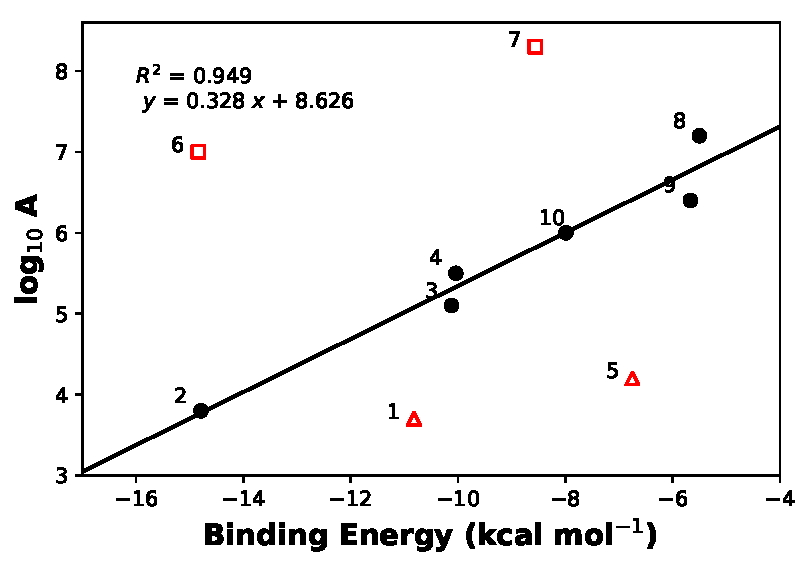
\includegraphics[width=0.75\textwidth]{figures/arrhenius-scatter.pdf}
  \caption[bleh]{bleh}
\label{fig:Arrhenius}
\end{figure}

\section{Discussion}



\section{Computational methods and details}

Density-functional theory (DFT) calculations were carried out using the Gaussian-09 software package.\cite{Frisch2009} Care was taken to obtain minimum energy structures through detailed conformational analysis. For this, I utilised the BLYP density-functional\cite{Becke1988,Lee1988} paired with the emprical D3 dispersion correction\cite{Grimme2010} with the recommended Becke-Johnson damping functions,\cite{Johnson2006} as well as our groups own \emph{basis set incompletion potentials} (BSIPs),$^*$\jnote{update citation} and the minimal MINIs basis sets.\cite{Huzinaga1984} The use of minimal basis sets corrected for basis set incompleteness allows DFT-based methods (as opposed to semi-empirical or force-field based approached) to be used to efficently perform a large number of calculations. Minimum energy geometries of the monomers (substrates and radicals) were first obtained by manual manipulation of the necessary dihedral bond angles, followed by geometry optimisation and vibrational analysis.

The lowest energy substrates were combined to generate the appropriate pre-reaction complexes. These pre-reaction complexes were subject to conformational analysis using the same BLYP-D3(BJ)-BSIP/MINIs method. Geometries were initially manipulated by hand. It became apparent that manual manipulation resulted in an unsatisfactory exploration of the conformational space. To solve this, all the necessary dihedral angles were scanned systematically using a combination of scripts.\cite{note5} All manipulated geometries were subject to optimisation. For each complex, the top 5--10 complex geometries were subject to further optimisation using a higher level of theory (BLYP-D3(BJ)/pc-1) to obtain the final minimum energy pre-reaction complex structures. Due to the free rotation of \emph{tert}-butyl and methyl groups, some of the optimised pre-reaction complex structures contain small imaginary frequencies, and thus do not represent proper stationary states. Several measures were taken to resolve this, however, no resolution was obtained. Regardless, the complexes adequately represent the pre-reaction complex and differences in ``true'' binding energies should be negligible.

To obtain accurate pre-reaction complex binding energies, the substrates and complexes were subject to single-point energy calculations using the LC-$\omega$PBE long-range corrected density functional\cite{Vydrov2006,Vydrov2006a} with D3(BJ) dispersion corrections and pc-2 basis sets with truncated $f$-type functions (pc-2-spd).\cite{Johnson2013} This method was selected on the recommendation of work by \citet{Johnson2013}, which demonstrated that this is an efficient method for the calculation of NCIs with a reasonable degree of accuracy.
